\documentclass{article}
\usepackage[utf8]{inputenc}
\usepackage[icelandic]{babel}
\usepackage[T1]{fontenc}
\usepackage{graphicx}
\usepackage{mathtools}
\usepackage{amsmath}
\usepackage{amssymb}
\usepackage{minted}


\graphicspath{ {./} }
\title{Bingó - Viðmótsforritun}
\author{ttb3@hi.is}
\date{\today}


\begin{document}
\maketitle

Þegar forritið er keyrt opnast gluggi með einum takka\\
\begin{center}
    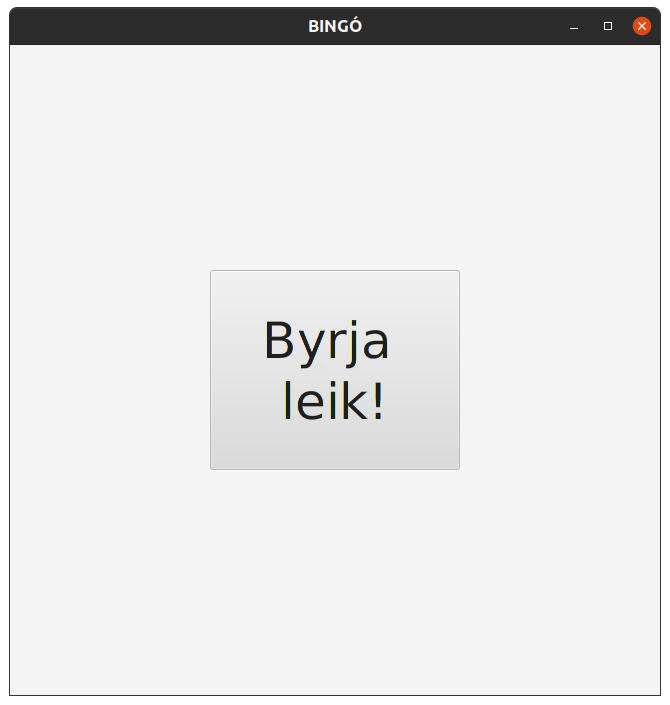
\includegraphics[scale=0.25]{1.png}
\end{center}
þegar smellt er á takkan birtist nýtt bingóspjald, þetta spjald er alltaf random, talan á hverjum reit fylgir reglunum um bingó\\
\begin{center}
    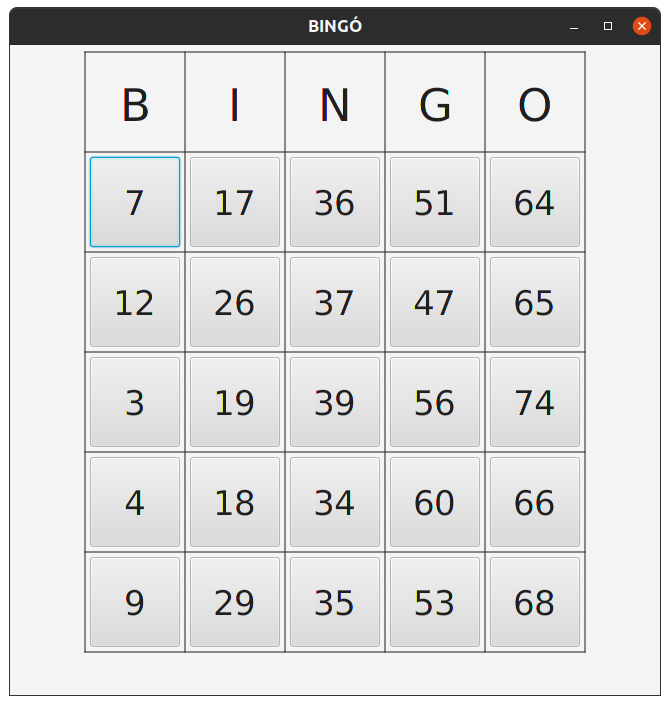
\includegraphics[scale=0.25]{9.png}
    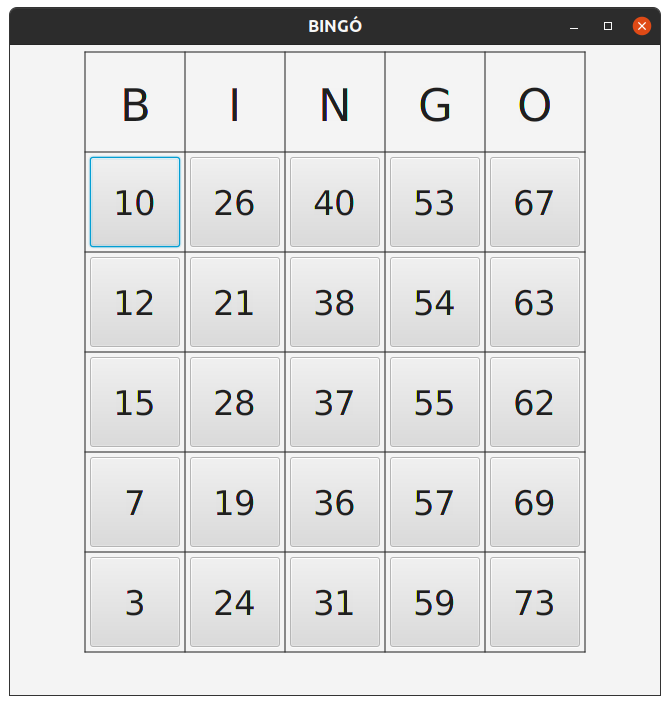
\includegraphics[scale=0.25]{8.png}
    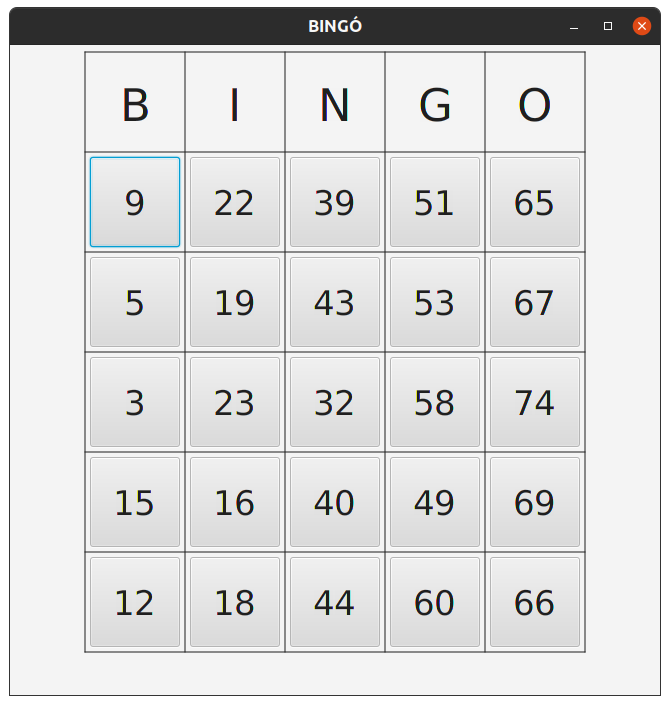
\includegraphics[scale=0.25]{2.png}
\end{center}
hægt er að smella á hvern reit og "merkja" hann, eftir að reitur er merktur er takkinn óvirkur
\begin{center}
    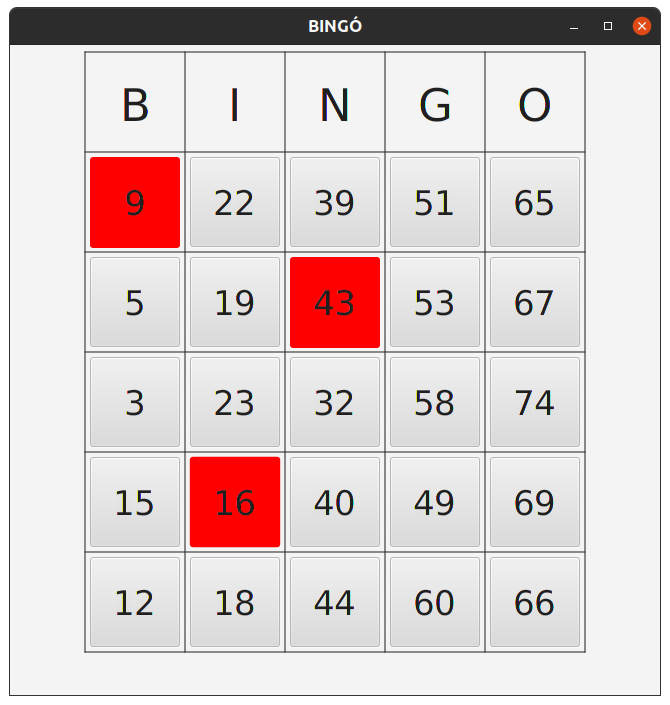
\includegraphics[scale=0.25]{3.png}
\end{center}
forritið tekur eftir því hvort að maður sé með bingó á lóðrétta, lárétta, ská niður og ská upp ásunum og lætur mann vita þegar maður fær bingó ásamt því að segja hvernig bingó það var\\
\begin{center}
    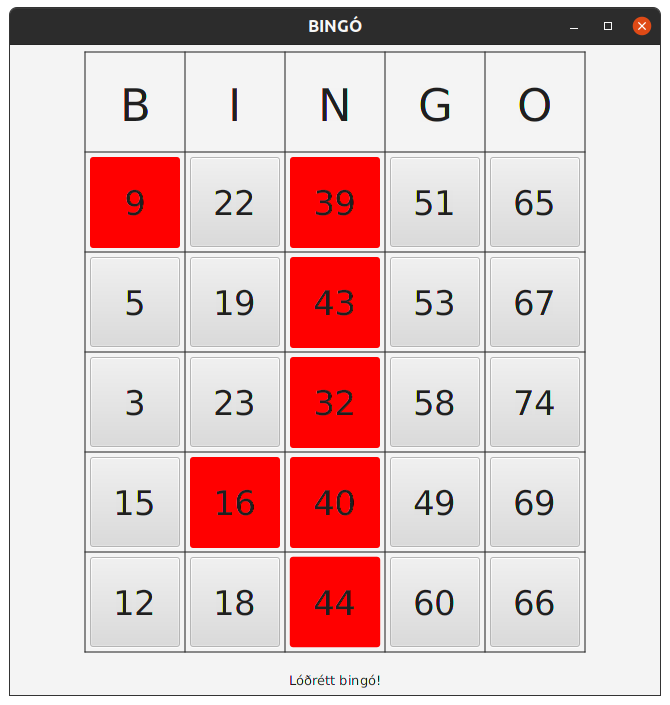
\includegraphics[scale=0.25]{4.png}
    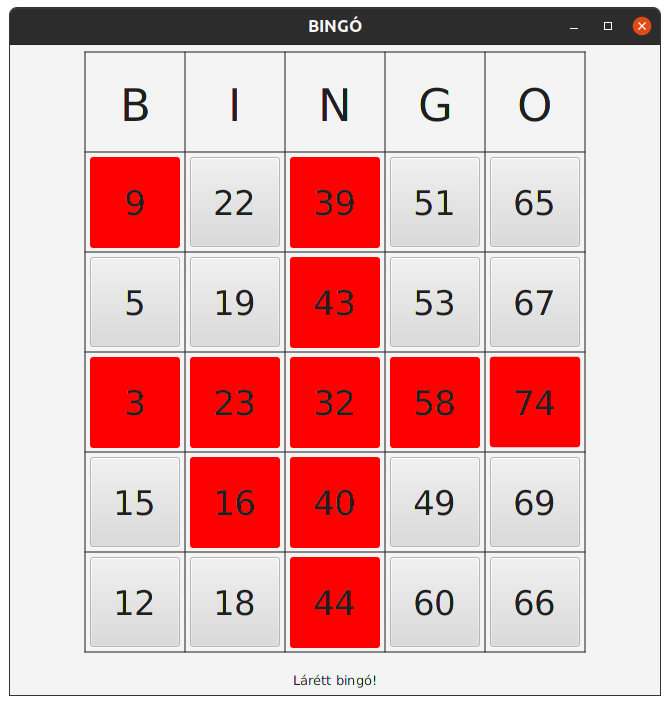
\includegraphics[scale=0.25]{5.png}
    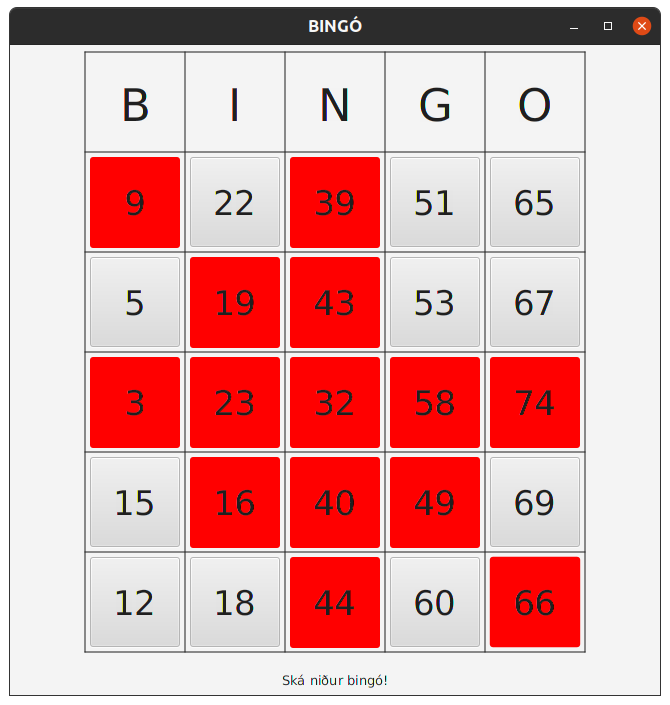
\includegraphics[scale=0.25]{6.png}
    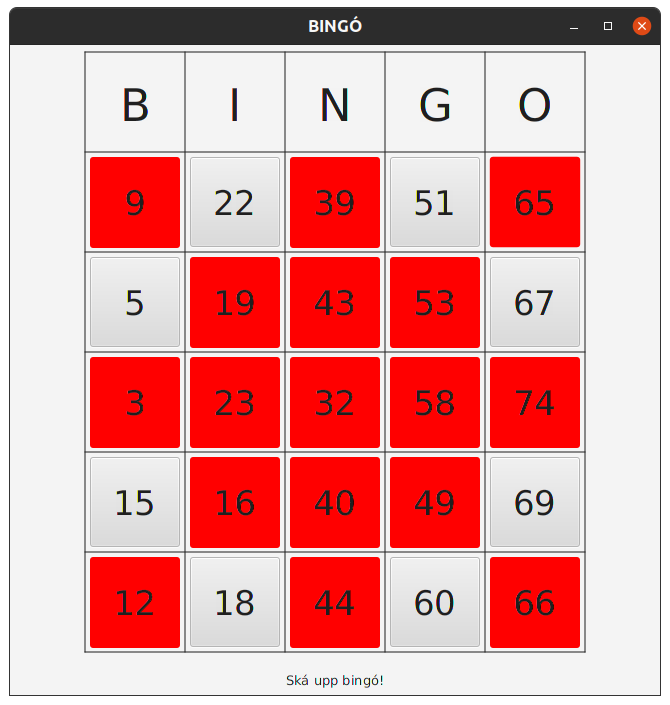
\includegraphics[scale=0.25]{7.png}
\end{center}

\end{document}